\documentclass{llncs}

\usepackage{llncsdoc}
\usepackage{graphicx,url}
\usepackage[USenglish]{babel}
\usepackage[utf8]{inputenc}
\usepackage{float}
\usepackage{setspace}

\usepackage{tabularx}
\usepackage{cite}
\usepackage{hyperref}
\usepackage{subcaption}

\begin{document}
\sloppy
\title{Mezuro: Understading source code metrics}

\author{Dylan Guedes\inst{1}, Paulo Meirelles\inst{1,2},
        Rafael Manzo\inst{2}, Diego Camarinha\inst{2}}


\institute{Faculdade do Gama -- Universidade de Brasília (UnB)\\
  Área Especial de Indústria Projeção A -- Setor Leste -- Gama -- DF -- Brazil \\
  \email{120115727@aluno.unb.br,paulormm@unb.br}
  \and
  Instituto de Matemática e Estatística -- Universidade de São Paulo (USP)\\
  Rua do Matão, 1010 -- 05508-090 -- Cidade Universitária -- São Paulo -- SP -- Brasil\\
  \email{\{paulormm,manzo,diegoamc\}@ime.usp.br}}

\maketitle
\begin{abstract}
  % Contexto
  The ease of development and maintenance of a software is directly related
with its source code quality.
  % Problema
  However, its analysis has issues like, for instance, the definition of which
metrics to use and how to interpret the measured results. Furthermore, this practice
is still not common on industry development workflow. Those who decide to employ
source code analysis lack free software alternatives that integrate multiple languages
and tools.
% Soluções propostas
In this work we present Mezuro: a FOSS web-based platform to collaboratively analyze
source code. The project provides ways to compare projects and share knowledge
about metrics, teaching how to configure and interpret them. The platform was
planned to integrate multiple metric collectors for several programming
languages, and, currently, allows analysis of source code written in C, C++,
Java, Ruby, PHP, and Python.
  % Frase de impacto
    With this project we expect to spread knowledge and encourage the use of
code metrics by the free software developer community.

\textbf{Keywords:} static analysis, source code metrics, open source software.
\end{abstract}

\section{Introduction}
\label{sec:intro}

Static source code metrics are measures extracted from the code without compiling
or running it. For example, these metrics provide information about complexity, comprehension,
testability, maintainability, and evolution of code \cite{mills1988}. Source code metrics can help software engineers to
observe and determine source code quality, supporting the development of clean code (i.e., clear, flexible, and simple) as well\cite{martin2008}.

Nowadays, several tools can be
used to extract source code metrics, such as
pylint\footnote{\url{http://www.pylint.org/}} (Python),
metric\_fu\footnote{\url{https://github.com/metricfu/metric_fu}} (Ruby), and
Analizo (C/C++ and Java)\cite{terceiro2010analizo}, each one with
different levels of usability, definitions and set of metrics, being necessary
the creation of a platform that brings and present these results to the end
user, specially in tracking the software during its life cycle.

Code metric tools, in general, do not present a friendly interface, and,
even more, do not follow a standard. Therefore, this work present the
Mezuro platform, which (i) provides an single interface grouping available tools;
(ii) allows selection and composition of metrics in a flexible manner;
(iii) preserves the evolution history;
(iv) presents results in a friendly way;
(v) allows users to customize the given interpretation accordingly to their own context.

\section{Related tools}

There are two tools related to Mezuro. The first, SonarQube\footnote{\url{http://www.sonarqube.org/}}, is a FOSS software licensed as LGPLv3, and offers a platform to manage software quality by using plugins through a 
library\footnote{\url{http://docs.codehaus.org/display/SONAR/Plugin+Library/}}.
At its most basic version it classifies code problems and evaluate simple
coverage metrics and technical debts in several languages. However, its best
plugins are paid and closed source, such as the
C/C++ analyzer\footnote{\url{http://www.sonarsource.com/products/plugins/languages/cpp/}}.

The second, Code Climate\footnote{\url{https://codeclimate.com/}}, is a tool
that analysis source code hosted in a Git server, and has support for several
programming languages and frameworks. The analysis will look for code smells
in the code and classify them based on aspects such as size of methods and
code duplication. Lastly, based on the score of its parts, the given project
will receive a grade between A and F. Keep in mind that what is tagged as an
issue sometimes is not a real problem, since it could be the best solution for
the given scenario.

Mezuro, idealized as a code metrics platform, has the differential to
continuous generate reviews about the project: the user schedule the
analysis and follows scores evolution over time. Results of each analysis
are public, what allows greater transparency between the developer and the
community that uses the software. Thereby, they can decide if the given solution
meets the requirements and if they should trust in the quality of the software.

\section{The Mezuro project}
\label{sec:mezuro}

Mezuro is composed of three parts: the configuration prior to the analysis beginning;
processing and evaluation of source code metrics; and a graphic interface to
present results. Nowadays, the processing module is Kalibro and the visualization
Prezento, Mezuro being so the set of these projects, that is, Kalibro integrated
with Prezento.

Since its first implementation in 2010\cite{mezuro2012}, until being completely
rewritten, the architecture of the system evolved adopting the microservice architecture\cite{namiot2014micro},
to (i) minimize the amount of code to maintain;
(ii) test and grant quality of code;
(iii) modularize the application in several independent services.

\begin{figure}[hbt]
  \centering
    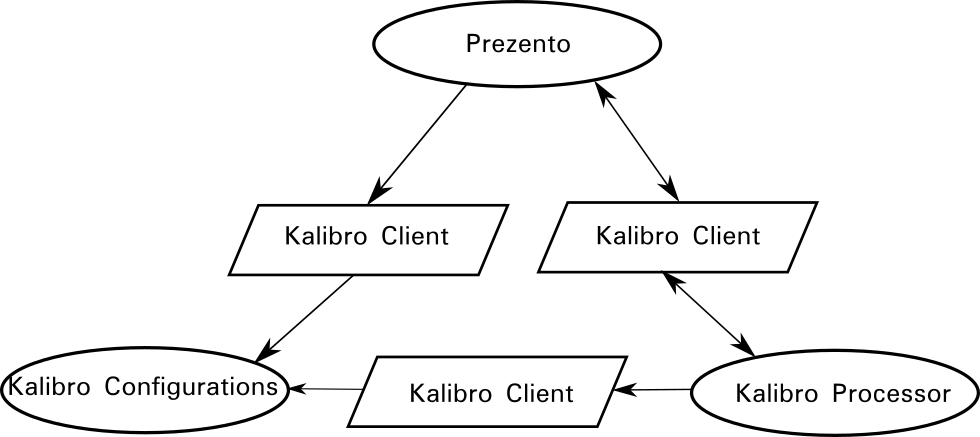
\includegraphics[width=\textwidth]{images/mezuro-architecturev3.png}
  \caption{Current architecture of the system.}
  \label{fig:architecture-2}
\end{figure}

%TODO Dylan: Possivelmente essa figura não é mais do estado atual - ver com o Manzo e Diego.

The current Mezuro state is specified on Figure \ref{fig:architecture-2}. Ellipses represents
softwares involved and parallelograms the communication interfaces between them. At Mezuro's
base we have Kalibro, segmented in three smaller entities (...).

Mezuro features can be divided in two groups:

\begin{itemize}
    \item Project

    \begin{itemize}
        \item Download of source code via repositories (Git, Subversion, Bazaar etc) or via compressed file;
        \item Scheduling of code processing (1 day, 2 days, weekly, biweekly, and monthly);
        \item Definition of what metric configuration should be used for each file;
        \item Graphical analysis of each file via dotted plot with scores over time;
        \item Public results that are accessible by the community.
    \end{itemize}
    \item Configuration
    \begin{itemize}
        \item Configuration cloning and creation;
        \item Statistics about most popular configurations in the community;
        \item Creation of qualitative ranges associated with values of metrics;
        \item Creation of reading groups to be used in textual interpretation of metrics results;
        \item Combination of native metrics to create composed and more complex analysis.
    \end{itemize}
\end{itemize}

\begin{figure}[H]
    \centering
    \begin{minipage}{.5\textwidth}
        \centering
        \includegraphics[width=.9\linewidth]{images/mezuro-feature1.png}
        % \caption{Feature 1}
        \captionof{figure}{Code analysis feature.}
        \label{fig:feature-1}
    \end{minipage}%
    \begin{minipage}{.5\textwidth}
        \centering
        \includegraphics[width=.9\linewidth]{images/mezuro-feature2.png}
        \captionof{figure}{Configuration creation feature.}
        \label{fig:feature-2}
    \end{minipage}
\end{figure}

%TODO Dylan: Adicionar duas imagens do Mezuro, a lado a lado

Mezuro has a social network shape, in which participants can observe other
projects, or clone their configurations and definitions. This open mutual
interaction can be interesting to project managers, software
auditors and even an entire developer team. The final goal is to create a
community that see value in such methodologies and how this can contribute
to the success of their projects.

\section{Final remarks}

Mezuro architecture evolution is an answer to the lack of tracking and standardization
of source code and the necessity to evaluate it, while being free software,
highly customizable, with support to many programming languages, providing
a friendly interface, for processing history and also with an extensible
architecture planned to easily embodying of new features by the FOSS community.

%TODO Paulo: mais coisas ...

\bibliographystyle{splncs03}
\bibliography{mezuro}
\end{document}
